\chapter{Arhitektura i dizajn sustava}
		
		\textbf{\textit{dio 1. revizije}}\\

		\textit{ Potrebno je opisati stil arhitekture te identificirati: podsustave, preslikavanje na radnu platformu, spremišta podataka, mrežne protokole, globalni upravljački tok i sklopovsko-programske zahtjeve. Po točkama razraditi i popratiti odgovarajućim skicama:}
	\begin{itemize}
		\item 	\textit{izbor arhitekture temeljem principa oblikovanja pokazanih na predavanjima (objasniti zašto ste baš odabrali takvu arhitekturu)}
		\item 	\textit{organizaciju sustava s najviše razine apstrakcije (npr. klijent-poslužitelj, baza podataka, datotečni sustav, grafičko sučelje)}
		\item 	\textit{organizaciju aplikacije (npr. slojevi frontend i backend, MVC arhitektura) }		
	\end{itemize}

	
		

		

				
		\section{Baza podataka}
			
			\textbf{\textit{dio 1. revizije}}\\
			
		U našem projektu odabrali smo PostgrSQL kao susatav za upravljanje bazama podataka. Implementacija naše PostgrSQL baze podataka obuhvaća nekoliko ključnih elemenata, uključujući organizaciju podataka u tablicama i uspostavljanje veza između tablica radi složenih upita. Baza podatka sastoji se od slijedećih entiteta: 
		
		\begin{packed_item}
			\item KLINIKA
			\item SMJEŠTAJ
			\item PRIJEVOZNIK
			\item VOZILO
			\item KORISNIK
			\item PUTOVANJE
		\end{packed_item}
		
			\subsection{Opis tablica}
			
				\textbf{KLINIKA}\hspace{0.5cm}Entitet KLINIKA sadrži informacije o ID-u klinike, nazivu i adresi. Prema tome, entitet KLINIKA posjeduje sljedeće atribute: IDKlinika, naziv i adresa. Entitet KLINIKA u vezi je \textit{One-to-Many} s entitetom SMJESTAJ preko atributa IDKlinika i u vezi \textit{One-to-Many} s enitetom PUTOVANJE preko atributa IDKlinika. Također je u \textit{One-to-Many} vezi s enitetom PUTOVANJE preko atributa adresa.
				
				\begin{longtblr}[
					label=none,
					entry=none
					]{
						width = \textwidth,
						colspec={|X[6,l]|X[6, l]|X[20, l]|}, 
						rowhead = 1,
					} %definicija širine tablice, širine stupaca, poravnanje i broja redaka naslova tablice
					\hline \SetCell[c=3]{c}{\textbf{KLINIKA}}	 \\ \hline[3pt]
					\SetCell{LightGreen}IDKlinika & INT	& Identifikacijski ključ klinike	\\ \hline
					naziv	& VARCHAR & Naziv klinike\\ \hline 
					adresa & VARCHAR & Adresa klinike\\ \hline 
				\end{longtblr}
				
				\textbf{SMJESTAJ}\hspace{0.5cm}Entitet SMJESTAJ sadrži podatke o ID-u smještaja, tipu stana, kategoriji opremljenosti, adresi kao i vremenskom periodu dostupnosti za korištenje. Sukladno tome, entitet SMJESTAJ posjeduje sljedeće atribute: IDSmjestaj, tip, kategorija, adresa i dostupnost. Entiet SMJESTAJ u vezi je  \textit{Many-to-One} s entitetom KLINIKA preko atributa IDKlinika i u vezi  \textit{One-to-Many} s enitetom PUTOVANJE preko atributa IDPutovanje. Također je u \textit{One-to-Many} vezi s enitetom PUTOVANJE preko atributa adresa.
				
				\begin{longtblr}[
					label=none,
					entry=none
					]{
						width = \textwidth,
						colspec={|X[6,l]|X[6, l]|X[20, l]|}, 
						rowhead = 1,
					} %definicija širine tablice, širine stupaca, poravnanje i broja redaka naslova tablice
					\hline \SetCell[c=3]{c}{\textbf{SMJESTAJ}}	 \\ \hline[3pt]
					\SetCell{LightGreen}IDSmjestaj & INT	&  Identifikacijski ključ smještaja	\\ \hline
					tip	& VARCHAR &  Tip stana\\ \hline 
					kategorija & VARCHAR & Kategorija opremljenosti  \\ \hline 
					adresa & VARCHAR	&  Adresa smještaja\\ \hline 
					dostupnost & INTERVAL	&  Vremenski period dostupnosti za korištenje\\ \hline 
					\SetCell{LightBlue} IDKlinika & INT	&  Identifikacijski ključ klinike  	\\ \hline 
				\end{longtblr}
				
				\textbf{PRIJEVOZNIK}\hspace{0.5cm}Entitet PRIJEVOZNIK sadrži informacije o ID-u prijevoznika, kontaktnim podacima i o radnom vremenu u kojem je prijevoznik raspoloživ. Prema tome, entitet PRIJEVOZNIK posjeduje sljedeće atribute: IDPrijevoznik, kontakt i radnoVrijeme. Entitet PRIJEVOZNIK u vezi je \textit{One-to-Many} s entitetom VOZILO preko atributa IDPrijevoznik i u vezi \textit{One-to-Many} s enitetom PUTOVANJE preko atributa IDPrijevoznik.
				
				
				\begin{longtblr}[
					label=none,
					entry=none
					]{
						width = \textwidth,
						colspec={|X[6,l]|X[6, l]|X[20, l]|}, 
						rowhead = 1,
					} %definicija širine tablice, širine stupaca, poravnanje i broja redaka naslova tablice
					\hline \SetCell[c=3]{c}{\textbf{PRIJEVOZNIK}}	 \\ \hline[3pt]
					\SetCell{LightGreen}IDPrijevoznik & INT	& Identifikacijski ključ prijevoznika	\\ \hline
					kontakt	& VARCHAR &  Kontaktni podatci prijevoznika	\\ \hline 
					radnoVrijeme & TIME & Radno vrijeme u kojem su prijevoznici raspoloživi  \\ \hline 
				\end{longtblr}
				
				\textbf{VOZILO}\hspace{0.5cm}Entitet VOZILO sadrži informacije o ID-u vozila, vrsti i kapacitetu prijevoznog sredstva. Prema tome, entitet VOZILO posjeduje sljedeće atribute: IDVozilo, vrsta i kapacitet. Entitet VOZILO u vezi je \textit{Many-to-One} s entitetom PRIJEVOZNIK preko atributa IDPrijevoznik.
				
				\begin{longtblr}[
					label=none,
					entry=none
					]{
						width = \textwidth,
						colspec={|X[6,l]|X[6, l]|X[20, l]|}, 
						rowhead = 1,
					} %definicija širine tablice, širine stupaca, poravnanje i broja redaka naslova tablice
					\hline \SetCell[c=3]{c}{\textbf{VOZILO}}	 \\ \hline[3pt]
					\SetCell{LightGreen}IDVozilo & INT	&  Identifikacijski ključ vozila	\\ \hline
					vrsta	& VARCHAR & Vrsta vozila\\ \hline 
					kapacitet & VARCHAR & Kapacitet vozila\\ \hline 
					\SetCell{LightBlue} IDPrijevoznik & INT	& Identifikacijski ključ prijevoznika   	\\ \hline 
				\end{longtblr}
				
				\textbf{KORISNIK}\hspace{0.5cm}Entitet KORISNIK sadrži informacije o ID-u korisnika, imenu, prezimenu, kontaktnim podacima i preferencijama vezanim uz veličinu i kvalitetu smještaja. Prema tome, entitet KORISNIK posjeduje sljedeće atribute: IDKorisnik, ime, prezime, kontakt i preferencije. Entitet KORISNIK u vezi je \textit{One-to-Many} s enitetom PUTOVANJE preko atributa IDKorisnik.
				
				\begin{longtblr}[
					label=none,
					entry=none
					]{
						width = \textwidth,
						colspec={|X[6,l]|X[6, l]|X[20, l]|}, 
						rowhead = 1,
					} %definicija širine tablice, širine stupaca, poravnanje i broja redaka naslova tablice
					\hline \SetCell[c=3]{c}{\textbf{KORISNIK}}	 \\ \hline[3pt]
					\SetCell{LightGreen}IDKorisnik & INT	&  Identifikacijski ključ korisnika	\\ \hline
					ime	& VARCHAR & Ime korisnika	\\ \hline 
					prezime & VARCHAR & Prezime korisnika \\ \hline
					kontakt & VARCHAR & Kontakt korisnika \\ \hline 
					preferencije & VARCHAR	& Preferencije vezane uz veličinu i kvalitetu smještaja\\ \hline 
				\end{longtblr}
				
				\textbf{PUTOVANJE}\hspace{0.5cm}Entitet PUTOVANJE sadrži informacije o ID-u putovanja, vremenu i smjeru putovanja. Prema tome, entitet PUTOVANJE posjeduje sljedeće atribute: IDPutovanje, vrijeme i smjer. Entitet PUTOVANJE u vezi je \textit{Many-to-One} s enitetom KLINIKA preko atributa IDKorisnik, u vezi \textit{Many-to-One} s enitetom SMJESTAJ preko atributa IDSmjestaj, u vezi \textit{Many-to-One} s enitetom KORISNIK preko atributa IDKorisnik, u vezi \textit{Many-to-One} s enitetom PRIJEVOZNIK preko atributa IDPrijevoznik. Atributi adresa1 i adresa2 su atributi iz kojih saznajemo adresu polaska ili dolaska u ovisnosti o smjeru koji može biti 1 ili 0. Entitet PUTOVANJE u vezi je \textit{Many-to-One} s enitetom KLINIKA preko atributa adresa1, u vezi \textit{Many-to-One} s enitetom SMJESTAJ preko atributa adresa2.
				
				\begin{longtblr}[
				label=none,
				entry=none
					]{
						width = \textwidth,
						colspec={|X[6,l]|X[6, l]|X[20, l]|}, 
						rowhead = 1,
					} %definicija širine tablice, širine stupaca, poravnanje i broja redaka naslova tablice
					\hline \SetCell[c=3]{c}{\textbf{PUTOVANJE}}	 \\ \hline[3pt]
					\SetCell{LightGreen}IDPutovanje & INT	&  Identifikacijski ključ putovanja	\\ \hline
					vrijeme	& TIME &  Vrijeme putovanja	\\ \hline 
					smjer & INT &  Smjer u kojem se putovanje izvodi \\ \hline 
					\SetCell{LightBlue} adresa1 & VARCHAR	&  Adresa klinike\\ \hline
					\SetCell{LightBlue} adresa2 & VARCHAR	& Adresa smještaja\\ \hline 
					\SetCell{LightBlue} IDKorisnik & INT	&  Identifikacijski ključ korisnika	\\ \hline 
					\SetCell{LightBlue} IDKlinika & INT	& Identifikacijski ključ klinike	\\ \hline
					\SetCell{LightBlue} IDPrijevoznik & INT	& Identifikacijski ključ prijevoznika	\\ \hline
					\SetCell{LightBlue} IDSmjestaj & INT	& Identifikacijski ključ smještaja	\\ \hline
				\end{longtblr}
				
			\eject
			
			\subsection{Dijagram baze podataka}
					
				\begin{figure}[htbp]
					\centering
					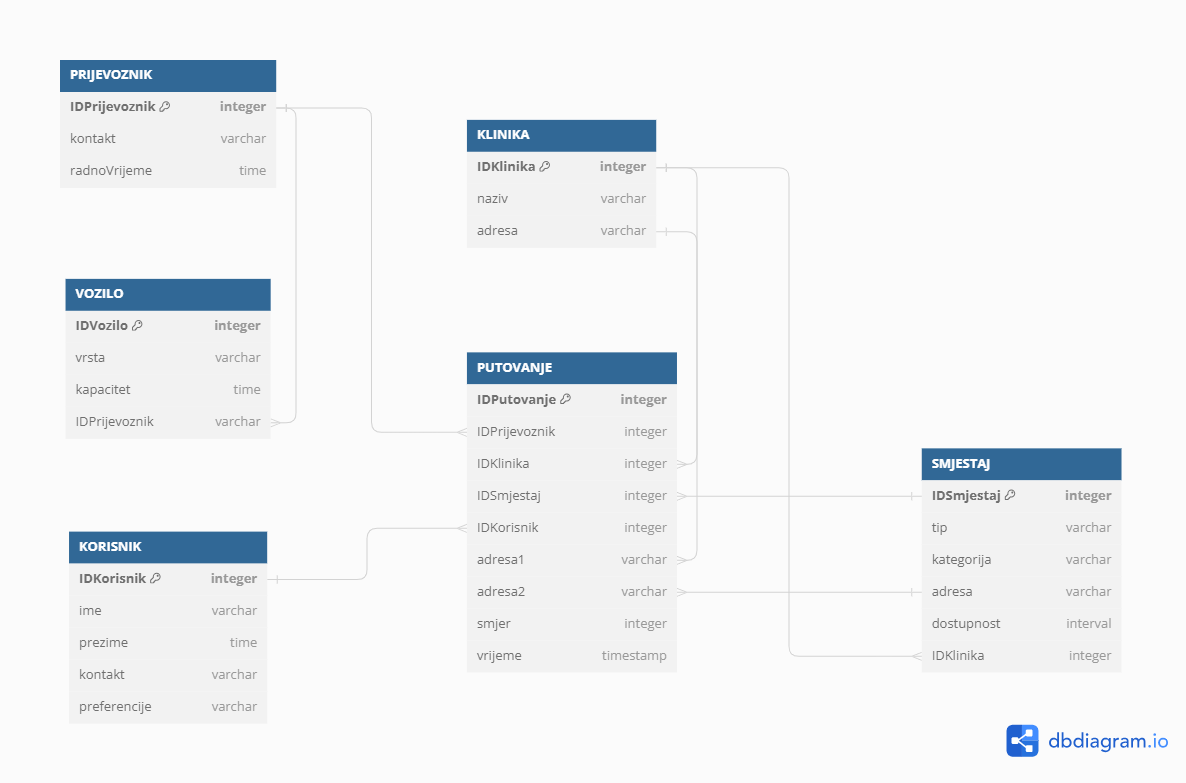
\includegraphics[width=0.9\textwidth]{slike/bazaPodataka.png}
					\caption{Relacijska shema baze podataka}
					\label{fig:bazaPodataka}
				\end{figure}
				
			
			\eject
			
			
		\section{Dijagram razreda}
		
			\textit{Potrebno je priložiti dijagram razreda s pripadajućim opisom. Zbog preglednosti je moguće dijagram razlomiti na više njih, ali moraju biti grupirani prema sličnim razinama apstrakcije i srodnim funkcionalnostima.}\\
			
			\textbf{\textit{dio 1. revizije}}\\
			
			\textit{Prilikom prve predaje projekta, potrebno je priložiti potpuno razrađen dijagram razreda vezan uz \textbf{generičku funkcionalnost} sustava. Ostale funkcionalnosti trebaju biti idejno razrađene u dijagramu sa sljedećim komponentama: nazivi razreda, nazivi metoda i vrste pristupa metodama (npr. javni, zaštićeni), nazivi atributa razreda, veze i odnosi između razreda.}\\
			
			\textbf{\textit{dio 2. revizije}}\\			
			
			\textit{Prilikom druge predaje projekta dijagram razreda i opisi moraju odgovarati stvarnom stanju implementacije}
			
			
			
			\eject
		
		\section{Dijagram stanja}
			
			
			\textbf{\textit{dio 2. revizije}}\\
			
			\textit{Potrebno je priložiti dijagram stanja i opisati ga. Dovoljan je jedan dijagram stanja koji prikazuje \textbf{značajan dio funkcionalnosti} sustava. Na primjer, stanja korisničkog sučelja i tijek korištenja neke ključne funkcionalnosti jesu značajan dio sustava, a registracija i prijava nisu. }
			
			
			\eject 
		
		\section{Dijagram aktivnosti}
			
			\textbf{\textit{dio 2. revizije}}\\
			
			 \textit{Potrebno je priložiti dijagram aktivnosti s pripadajućim opisom. Dijagram aktivnosti treba prikazivati značajan dio sustava.}
			
			\eject
		\section{Dijagram komponenti}
		
			\textbf{\textit{dio 2. revizije}}\\
		
			 \textit{Potrebno je priložiti dijagram komponenti s pripadajućim opisom. Dijagram komponenti treba prikazivati strukturu cijele aplikacije.}